\documentclass{article}

\usepackage{arxiv}

\usepackage[utf8]{inputenc} % allow utf-8 input
\usepackage[T1]{fontenc}    % use 8-bit T1 fonts
\usepackage{lmodern}        % https://github.com/rstudio/rticles/issues/343
\usepackage{hyperref}       % hyperlinks
\usepackage{url}            % simple URL typesetting
\usepackage{booktabs}       % professional-quality tables
\usepackage{amsfonts}       % blackboard math symbols
\usepackage{nicefrac}       % compact symbols for 1/2, etc.
\usepackage{microtype}      % microtypography
\usepackage{graphicx}

\title{COMPAS Analysis - A Causal Approach}

\author{
    Drago Plecko
   \\
    Seminar for Statistics \\
    ETH Zurich \\
   \\
  \texttt{\href{mailto:drago.plecko@stat.math.ethz.ch}{\nolinkurl{drago.plecko@stat.math.ethz.ch}}} \\
   \And
    Elias Bareinboim
   \\
    Department of Computer Science \\
    Columbia University \\
   \\
  \texttt{\href{mailto:eb@cs.columbia.edu}{\nolinkurl{eb@cs.columbia.edu}}} \\
  }

% Pandoc syntax highlighting
\usepackage{color}
\usepackage{fancyvrb}
\newcommand{\VerbBar}{|}
\newcommand{\VERB}{\Verb[commandchars=\\\{\}]}
\DefineVerbatimEnvironment{Highlighting}{Verbatim}{commandchars=\\\{\}}
% Add ',fontsize=\small' for more characters per line
\usepackage{framed}
\definecolor{shadecolor}{RGB}{248,248,248}
\newenvironment{Shaded}{\begin{snugshade}}{\end{snugshade}}
\newcommand{\AlertTok}[1]{\textcolor[rgb]{0.94,0.16,0.16}{#1}}
\newcommand{\AnnotationTok}[1]{\textcolor[rgb]{0.56,0.35,0.01}{\textbf{\textit{#1}}}}
\newcommand{\AttributeTok}[1]{\textcolor[rgb]{0.77,0.63,0.00}{#1}}
\newcommand{\BaseNTok}[1]{\textcolor[rgb]{0.00,0.00,0.81}{#1}}
\newcommand{\BuiltInTok}[1]{#1}
\newcommand{\CharTok}[1]{\textcolor[rgb]{0.31,0.60,0.02}{#1}}
\newcommand{\CommentTok}[1]{\textcolor[rgb]{0.56,0.35,0.01}{\textit{#1}}}
\newcommand{\CommentVarTok}[1]{\textcolor[rgb]{0.56,0.35,0.01}{\textbf{\textit{#1}}}}
\newcommand{\ConstantTok}[1]{\textcolor[rgb]{0.00,0.00,0.00}{#1}}
\newcommand{\ControlFlowTok}[1]{\textcolor[rgb]{0.13,0.29,0.53}{\textbf{#1}}}
\newcommand{\DataTypeTok}[1]{\textcolor[rgb]{0.13,0.29,0.53}{#1}}
\newcommand{\DecValTok}[1]{\textcolor[rgb]{0.00,0.00,0.81}{#1}}
\newcommand{\DocumentationTok}[1]{\textcolor[rgb]{0.56,0.35,0.01}{\textbf{\textit{#1}}}}
\newcommand{\ErrorTok}[1]{\textcolor[rgb]{0.64,0.00,0.00}{\textbf{#1}}}
\newcommand{\ExtensionTok}[1]{#1}
\newcommand{\FloatTok}[1]{\textcolor[rgb]{0.00,0.00,0.81}{#1}}
\newcommand{\FunctionTok}[1]{\textcolor[rgb]{0.00,0.00,0.00}{#1}}
\newcommand{\ImportTok}[1]{#1}
\newcommand{\InformationTok}[1]{\textcolor[rgb]{0.56,0.35,0.01}{\textbf{\textit{#1}}}}
\newcommand{\KeywordTok}[1]{\textcolor[rgb]{0.13,0.29,0.53}{\textbf{#1}}}
\newcommand{\NormalTok}[1]{#1}
\newcommand{\OperatorTok}[1]{\textcolor[rgb]{0.81,0.36,0.00}{\textbf{#1}}}
\newcommand{\OtherTok}[1]{\textcolor[rgb]{0.56,0.35,0.01}{#1}}
\newcommand{\PreprocessorTok}[1]{\textcolor[rgb]{0.56,0.35,0.01}{\textit{#1}}}
\newcommand{\RegionMarkerTok}[1]{#1}
\newcommand{\SpecialCharTok}[1]{\textcolor[rgb]{0.00,0.00,0.00}{#1}}
\newcommand{\SpecialStringTok}[1]{\textcolor[rgb]{0.31,0.60,0.02}{#1}}
\newcommand{\StringTok}[1]{\textcolor[rgb]{0.31,0.60,0.02}{#1}}
\newcommand{\VariableTok}[1]{\textcolor[rgb]{0.00,0.00,0.00}{#1}}
\newcommand{\VerbatimStringTok}[1]{\textcolor[rgb]{0.31,0.60,0.02}{#1}}
\newcommand{\WarningTok}[1]{\textcolor[rgb]{0.56,0.35,0.01}{\textbf{\textit{#1}}}}

% tightlist command for lists without linebreak
\providecommand{\tightlist}{%
  \setlength{\itemsep}{0pt}\setlength{\parskip}{0pt}}

% From pandoc table feature
\usepackage{longtable,booktabs,array}
\usepackage{calc} % for calculating minipage widths
% Correct order of tables after \paragraph or \subparagraph
\usepackage{etoolbox}
\makeatletter
\patchcmd\longtable{\par}{\if@noskipsec\mbox{}\fi\par}{}{}
\makeatother
% Allow footnotes in longtable head/foot
\IfFileExists{footnotehyper.sty}{\usepackage{footnotehyper}}{\usepackage{footnote}}
\makesavenoteenv{longtable}


\begin{document}
\maketitle


\begin{abstract}
In this submission, we analyze the COMPAS dataset from Broward County,
Florida. In particular, we expand the analysis of the COMPAS dataset
performed by ProPublica in 2016, by complementing the analysis with
tools of causal inference. Our analysis is performed in three steps.
Firstly, we compute the disparity between demographic groups in the
actual, true recidivism rates, and provide a \emph{causal explanation}
for how this disparity arose in practice. Secondly, we compute the
disparity between groups for the predictions produced by Northpointe,
Inc., and demonstrate that the predictions have a different causal
explanation, directly pointing to discrimination. Finally, in the last
step, we provide a causal explanation for the disparity of Northpointe's
predictions in the group of individuals who did not recidivate - which
shows once again that there is a discriminatory effect of race on the
predictions. The implication of our analysis is that there prima facie
evidence against Northpointe exists, who discriminated against minority
groups purely based on race (and not on other, race related features),
which is prohibited by the Equal Protection clause of the 14th
Amendment.
\end{abstract}

\keywords{
    COMPAS dataset
   \and
    Causal Inference
   \and
    Causal Fairness Analysis
   \and
    Graphical Models
  }

\hypertarget{introduction}{%
\section{Introduction}\label{introduction}}

Across United States, courts are using algorithms to predict which of
the defendants are likely to recidivate and re-offend. As is becoming
apparent in the literature on fair machine learning, algorithms a priori
do not have any ethical or moral values, and they are capable of
learning, or even amplifying the existing societal bias. If left
unattended, such algorithms could lead to the perpetuation of
unfairness, raising a serious concern about the impact of AI on socially
important questions.

In their seminal work from 2016 \cite{larson2016recidivism}, the team
from ProPublica (an independent, non-profit newsroom), analyzed data
from a commercial tool called Correctional Offender Management Profiling
for Alternative Sanctions (COMPAS), which was developed by Northpointe,
Inc.~(the company is today known as Equivant). The analysis was
performed on a large number of individuals from Broward County, Florida,
and compared the recidivism predictions produced by COMPAS with those
that actually occurred in practice. The findings of their analysis sent
alarm bells ringing to everyone concerned about issues of racial
injustice. In particular, the ProPublica team demonstrated, among other
things, that:

\begin{itemize}
\tightlist
\item
  black defendants who did not recidivate over a two-year period were
  nearly twice as likely to be classified as higher risk compared to
  their white counterparts,
\item
  white defendants who did recidivate over a two-year period were
  labeled as low risk twice as often as black re-offenders.
\end{itemize}

The above mentioned disparities observed by ProPublica are a starting
point of an important investigation. What their analysis did not
investigate is the \emph{causal explanation} of how the disparities
arose. In particular, using the language of causal models, we provide
such an explanation as follows. For the observed disparity between the
groups, we quantify how much of the disparity can be explained by:

\begin{enumerate}[label=(\roman*)]
  \item the direct causal effect of race on the outcome (not explained by other features),
  \item  the indirect causal effect of race on previous offenses and degree of charge, which in turn influence the likelihood of recidivism,
  \item the confounded effect of race, which is associated with age and sex in the dataset.
\end{enumerate}

We remark here that our causal analysis should be thought of
manipulating the ``signals'' of race, or its perception, rather than
race itself, which is an immutable characteristic of every individual
\cite{weinberger2022signal, greiner2011causal}.

The three steps of our analysis are the following:

\begin{enumerate}[label=(\Alph*)]
  \item we first look at the causal explanation of the two-year recidivism rates $Y$, which will help us understand the causal effects of race in the real world,
  \item  we then look at the causal explanation of the Northpointe's predictions, which will help us understand the causal effects of the \textit{predicted world},
  \item finally, we look at the causal explanation of the Northpointe's predictions when subsetting to only the group of individuals who did not recidivate over a two-year period; such an analysis will help us understand how Northpointe's predictions causally treat individuals who do not re-offend.
\end{enumerate}

We now introduce the methodology used in our analysis, which is
implemented in the \texttt{faircause} R-package. The package can be
installed using:

\begin{Shaded}
\begin{Highlighting}[]
\NormalTok{devtools}\SpecialCharTok{::}\FunctionTok{install\_github}\NormalTok{(}\StringTok{"dplecko/CFA"}\NormalTok{)}
\end{Highlighting}
\end{Shaded}

\hypertarget{methodology}{%
\section{Methodology}\label{methodology}}

In this manuscript, we analyze the same COMPAS dataset as the ProPublica
team. tools of causal reasoning \cite{pearl:2k}. In particular, we
follow the approach of Causal Fairness Analysis described in
\cite{plecko2022causal}. First, we start by constructing a causal
graphical model of the dataset. The dataset consists of the following
information:

\begin{itemize}
\tightlist
\item
  the protected attribute \(X\), in this case race (for simplicity, race
  has two levels, corresponding to the majority group, and all other
  minority groups put together),
\item
  the confounding variables \(Z\), in this case age and sex,
\item
  the mediator variables \(W\), in this chase juvenile and prior offense
  counts, and the charge of degree,
\item
  two outcome variables, \(Y\) and \(\hat{Y}\), which represent the
  two-year recidivism and the Northpointe's prediction, respectively.
\end{itemize}

Therefore, our dataset looks like:

\begin{longtable}[]{@{}
  >{\raggedright\arraybackslash}p{(\columnwidth - 18\tabcolsep) * \real{0.0581}}
  >{\raggedleft\arraybackslash}p{(\columnwidth - 18\tabcolsep) * \real{0.0465}}
  >{\raggedright\arraybackslash}p{(\columnwidth - 18\tabcolsep) * \real{0.1047}}
  >{\raggedleft\arraybackslash}p{(\columnwidth - 18\tabcolsep) * \real{0.0930}}
  >{\raggedleft\arraybackslash}p{(\columnwidth - 18\tabcolsep) * \real{0.1047}}
  >{\raggedleft\arraybackslash}p{(\columnwidth - 18\tabcolsep) * \real{0.1163}}
  >{\raggedleft\arraybackslash}p{(\columnwidth - 18\tabcolsep) * \real{0.0814}}
  >{\raggedright\arraybackslash}p{(\columnwidth - 18\tabcolsep) * \real{0.0814}}
  >{\raggedleft\arraybackslash}p{(\columnwidth - 18\tabcolsep) * \real{0.1744}}
  >{\raggedleft\arraybackslash}p{(\columnwidth - 18\tabcolsep) * \real{0.1395}}@{}}
\caption{COMPAS dataset}\tabularnewline
\toprule
\begin{minipage}[b]{\linewidth}\raggedright
sex
\end{minipage} & \begin{minipage}[b]{\linewidth}\raggedleft
age
\end{minipage} & \begin{minipage}[b]{\linewidth}\raggedright
race
\end{minipage} & \begin{minipage}[b]{\linewidth}\raggedleft
juv\_fel
\end{minipage} & \begin{minipage}[b]{\linewidth}\raggedleft
juv\_misd
\end{minipage} & \begin{minipage}[b]{\linewidth}\raggedleft
juv\_other
\end{minipage} & \begin{minipage}[b]{\linewidth}\raggedleft
priors
\end{minipage} & \begin{minipage}[b]{\linewidth}\raggedright
charge
\end{minipage} & \begin{minipage}[b]{\linewidth}\raggedleft
two\_year\_recid
\end{minipage} & \begin{minipage}[b]{\linewidth}\raggedleft
northpointe
\end{minipage} \\
\midrule
\endfirsthead
\toprule
\begin{minipage}[b]{\linewidth}\raggedright
sex
\end{minipage} & \begin{minipage}[b]{\linewidth}\raggedleft
age
\end{minipage} & \begin{minipage}[b]{\linewidth}\raggedright
race
\end{minipage} & \begin{minipage}[b]{\linewidth}\raggedleft
juv\_fel
\end{minipage} & \begin{minipage}[b]{\linewidth}\raggedleft
juv\_misd
\end{minipage} & \begin{minipage}[b]{\linewidth}\raggedleft
juv\_other
\end{minipage} & \begin{minipage}[b]{\linewidth}\raggedleft
priors
\end{minipage} & \begin{minipage}[b]{\linewidth}\raggedright
charge
\end{minipage} & \begin{minipage}[b]{\linewidth}\raggedleft
two\_year\_recid
\end{minipage} & \begin{minipage}[b]{\linewidth}\raggedleft
northpointe
\end{minipage} \\
\midrule
\endhead
Male & 69 & Minority & 0 & 0 & 0 & 0 & F & 0 & 0 \\
Male & 34 & Minority & 0 & 0 & 0 & 0 & F & 1 & 0 \\
Male & 24 & Minority & 0 & 0 & 1 & 4 & F & 1 & 0 \\
Male & 23 & Minority & 0 & 1 & 0 & 1 & F & 0 & 1 \\
Male & 43 & Minority & 0 & 0 & 0 & 2 & F & 0 & 0 \\
Male & 44 & Minority & 0 & 0 & 0 & 0 & M & 0 & 0 \\
\bottomrule
\end{longtable}

The causal diagram of the above mentioned which is shown in Figure
\ref{fig:compas-sfm}, which shows how different variables influence each
other.

The causal graphical model can be interpreted as follows:

\begin{itemize}
\tightlist
\item
  there is a bidirected edge between race \(X\) and demographic
  variables \(Z\), which are correlated in the dataset; the edge
  represents either a confounding mechanism through some historical
  context, or a selection bias mechanism,
\item
  there is a directed edge from \(X\) to \(W\), \(Y\), which allows for
  the possibility that race has an effect on the prior offense counts,
  and the recidivism outcome; the edge can represent various types of
  bias, such as a bias in policing or the judicial system against
  minority groups.
\item
  there is a directed edge, from \(Z, W\) into the outcome \(Y\),
  allowing for the possibility that prior offense counts or demographic
  features influence recidivism,
\item
  there is a directed edge from \(Z\) to \(W\), which represents the
  effect of demographic variables on prior offense counts.
\end{itemize}

\begin{figure}
\centering
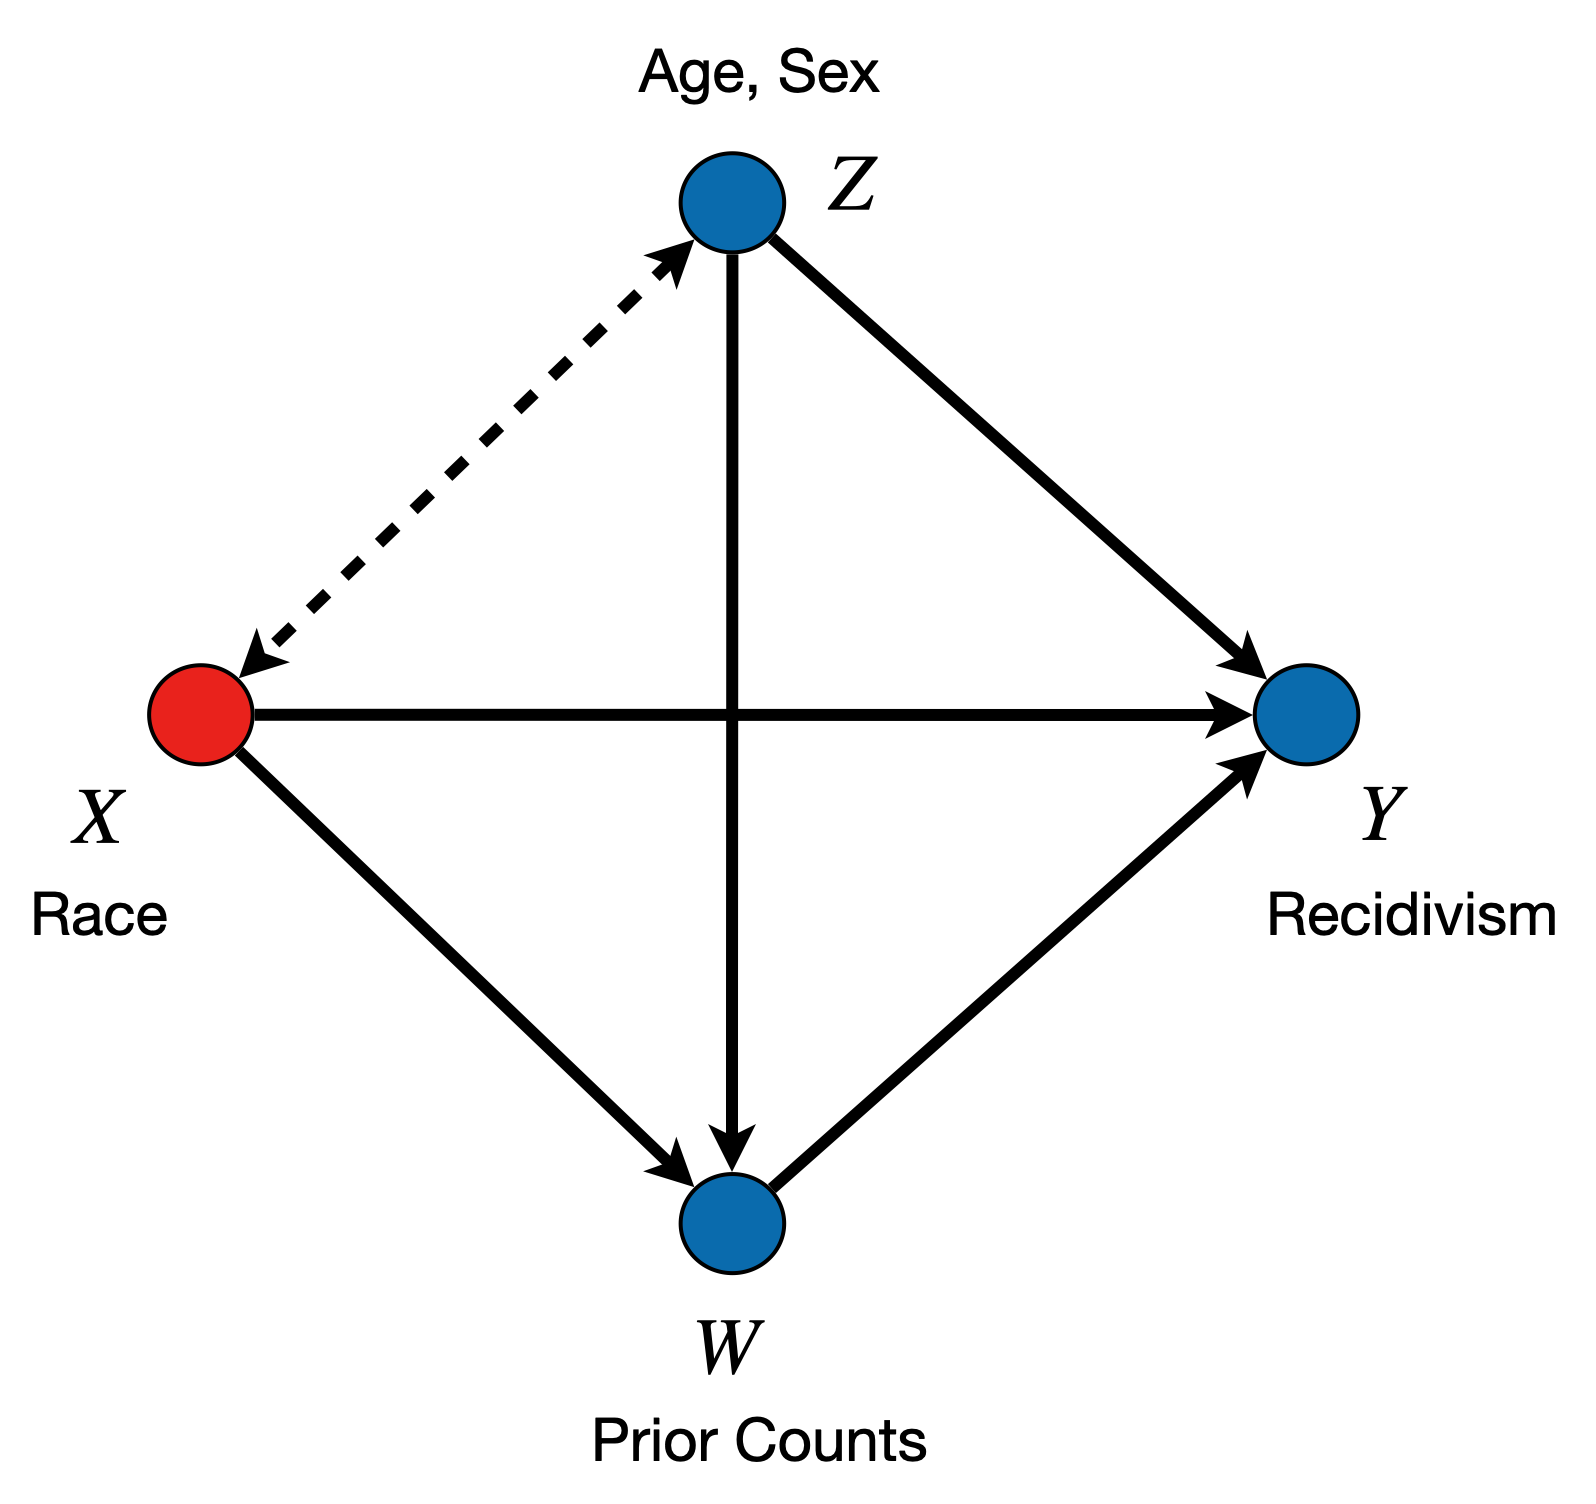
\includegraphics[width=5cm]{compas-sfm}
\caption{A causal model for the COMPAS dataset.}
\label{fig:compas-sfm}
\end{figure}

Based on the graphical model, and using the methodology of decomposing
variations described above, we can decompose the \emph{parity gap}
between the majority and minority groups, into its direct, indirect, and
confounded parts. The parity gap is defined as the difference in
conditional expectations between the groups, namely \begin{equation}
  \text{PG}_{x_0, x_1}(y) = P(Y = 1\mid X = x_1) - P(Y = 1 \mid X = x_0).
\end{equation}

Mathematically, we have the following equation decomposing the parity
gap:

\begin{equation}
  \text{PG}_{x_0, x_1}(y) = \underbrace{\text{DE}}_{\text{race effect}} +  \underbrace{\text{IE}}_{\text{prior counts effect}} +  \underbrace{\text{CE}}_{\text{age/sex effect}},
\end{equation} where DE, IE, and CE stand for direct, indirect, and
confounded effect respectively. After decomposing the parity gap for
two-year recidivism \(Y\), we also decompose it for the Northpointe's
predictions \(\hat{Y}\), and finally decompose it for the \(\hat{Y}\) in
the subgroup of individuals who did not recidivate (\(Y = 0\)).

\hypertarget{results}{%
\subsection{Results}\label{results}}

We now report on the results of our methodology of decomposing
variations. We report the results of the three experiments: A)
explaining the disparity in true recidivism; B) explaining disparity in
Northpointe's predictions; C) explaining disparity in Northpointe's
prediction for defendants who did not recidivate (\(Y = 0\)).

\hypertarget{a-explaining-disparity-in-recidivism}{%
\subsection{A: Explaining disparity in
recidivism}\label{a-explaining-disparity-in-recidivism}}

As our starting point, we first compute the disparity between groups in
two-year recidivism:

\begin{Shaded}
\begin{Highlighting}[]
\FunctionTok{tapply}\NormalTok{(data}\SpecialCharTok{$}\NormalTok{two\_year\_recid, data}\SpecialCharTok{$}\NormalTok{race, mean)}
\end{Highlighting}
\end{Shaded}

\begin{verbatim}
## Majority Minority 
## 0.393643 0.480042
\end{verbatim}

Based on this information, we can compute that: \begin{equation}
  \text{PG}_{x_0, x_1}(y) = 48\% - 39.5\% = 8.5\%.
\end{equation} We then apply the \texttt{fairness\_cookbook()}
functionality from the \texttt{faircause} R-package, and choose
\texttt{two\_year\_recid} (\(Y\)) as the outcome of interest:

\begin{Shaded}
\begin{Highlighting}[]
\NormalTok{X }\OtherTok{\textless{}{-}} \StringTok{"race"}
\NormalTok{Z }\OtherTok{\textless{}{-}} \FunctionTok{c}\NormalTok{(}\StringTok{"age"}\NormalTok{, }\StringTok{"sex"}\NormalTok{)}
\NormalTok{W }\OtherTok{\textless{}{-}} \FunctionTok{c}\NormalTok{(}\StringTok{"juv\_fel"}\NormalTok{, }\StringTok{"juv\_misd"}\NormalTok{, }\StringTok{"juv\_other"}\NormalTok{, }\StringTok{"priors"}\NormalTok{, }\StringTok{"charge"}\NormalTok{)}
\NormalTok{Y }\OtherTok{\textless{}{-}} \FunctionTok{c}\NormalTok{(}\StringTok{"two\_year\_recid"}\NormalTok{)}
\NormalTok{two\_year }\OtherTok{\textless{}{-}} \FunctionTok{fairness\_cookbook}\NormalTok{(data, }\AttributeTok{X =}\NormalTok{ X, }\AttributeTok{W =}\NormalTok{ W, }\AttributeTok{Z =}\NormalTok{ Z, }\AttributeTok{Y =}\NormalTok{ Y, }
                              \AttributeTok{x0 =} \StringTok{"Majority"}\NormalTok{, }\AttributeTok{x1 =} \StringTok{"Minority"}\NormalTok{)}
\NormalTok{two\_year}
\end{Highlighting}
\end{Shaded}

\begin{verbatim}
## faircause object:
## 
## Attribute:        race 
## Outcome:          two_year_recid 
## Confounders:      age,sex 
## Mediators:        juv_fel,juv_misd,juv_other,priors,charge
\end{verbatim}

After performing the decomposition we can visualize how the
decomposition works in practice:

\begin{Shaded}
\begin{Highlighting}[]
\FunctionTok{autoplot}\NormalTok{(two\_year, }\AttributeTok{decompose =} \StringTok{"xspec"}\NormalTok{, }\AttributeTok{signed =} \ConstantTok{FALSE}\NormalTok{)}
\end{Highlighting}
\end{Shaded}

\begin{figure}

{\centering \includegraphics[width=0.7\linewidth]{shai-challenge_files/figure-latex/vis-recid-1} 

}

\caption{Causal decomposition of the parity gap for two-year recidivism.}\label{fig:vis-recid}
\end{figure}

Therefore, we have the first crucial result: \begin{equation}
  \text{PG}_{x_0, x_1}(y) = \underbrace{1.5\%}_{\text{race effect}} +  \underbrace{4\%}_{\text{prior counts effect}} +  \underbrace{3\%}_{\text{age/sex effect}}.
\end{equation} Important to note is that \emph{race does not have a
statistically significant direct effect on outcome}.

\hypertarget{b-explaining-disparity-in-northpointes-recidivism-predictions}{%
\subsection{B: Explaining disparity in Northpointe's recidivism
predictions}\label{b-explaining-disparity-in-northpointes-recidivism-predictions}}

Our next step is to analyze the causal decomposition of the
Northpointe's predictions.

\begin{Shaded}
\begin{Highlighting}[]
\FunctionTok{tapply}\NormalTok{(data}\SpecialCharTok{$}\NormalTok{northpointe, data}\SpecialCharTok{$}\NormalTok{race, mean)}
\end{Highlighting}
\end{Shaded}

\begin{verbatim}
##  Majority  Minority 
## 0.3480033 0.5174370
\end{verbatim}

Therefore, we can compute that: \begin{equation}
  \text{PG}_{x_0, x_1}(\hat{y}) = 52\% - 35\% = 17\%.
\end{equation} Firstly, we notice that the disparity in the predicted
outcome is larger than in the true outcome. But crucially, the question
is how this disparity in predicted outcome arises from a causal point of
view. We again apply the \texttt{fairness\_cookbook()}, this time
choosing \texttt{northpointe} (\(\hat{Y}\)) as the outcome of interest:

\begin{Shaded}
\begin{Highlighting}[]
\NormalTok{Yhat }\OtherTok{\textless{}{-}} \StringTok{"northpointe"}
\NormalTok{north\_decompose }\OtherTok{\textless{}{-}} \FunctionTok{fairness\_cookbook}\NormalTok{(data, }\AttributeTok{X =}\NormalTok{ X, }\AttributeTok{W =}\NormalTok{ W, }\AttributeTok{Z =}\NormalTok{ Z, }\AttributeTok{Y =}\NormalTok{ Yhat, }
                                     \AttributeTok{x0 =} \StringTok{"Majority"}\NormalTok{, }\AttributeTok{x1 =} \StringTok{"Minority"}\NormalTok{)}
\FunctionTok{autoplot}\NormalTok{(north\_decompose, }\AttributeTok{decompose =} \StringTok{"xspec"}\NormalTok{, }\AttributeTok{signed =} \ConstantTok{FALSE}\NormalTok{) }\SpecialCharTok{+}
  \FunctionTok{ggtitle}\NormalTok{(}\FunctionTok{TeX}\NormalTok{(}\StringTok{"$PG\_\{x\_0, x\_1\}(}\SpecialCharTok{\textbackslash{}\textbackslash{}}\StringTok{hat\{y\})$ decomposition"}\NormalTok{))}
\end{Highlighting}
\end{Shaded}

\begin{figure}

{\centering \includegraphics[width=0.7\linewidth]{shai-challenge_files/figure-latex/north-cookbook-1} 

}

\caption{Causal decomposition of the parity gap for Northpointe's recidivism prediction.}\label{fig:north-cookbook}
\end{figure}

In particular, we obtain that: \begin{equation}
  \text{PG}_{x_0, x_1}(\hat{y}) = \underbrace{5.5\% \;(\pm 1.75\%)}_{\text{race effect}} +  \underbrace{7.5\% \;(\pm 1.2\%)}_{\text{prior counts effect}} +  \underbrace{3\%\;(\pm 1.5\%)}_{\text{age/sex effect}}.
\end{equation} Crucially, we find that \emph{race does have a
statistically significant direct effect on Northpointe's predictions}.
Furthermore, race by itself explains \emph{one third of the observed
disparity}.

\hypertarget{c-explaining-disparity-in-northpointes-recidivism-predictions-for-those-who-did-not-recidivate}{%
\subsection{\texorpdfstring{C: Explaining disparity in Northpointe's
recidivism predictions for \emph{those who did not
recidivate}}{C: Explaining disparity in Northpointe's recidivism predictions for those who did not recidivate}}\label{c-explaining-disparity-in-northpointes-recidivism-predictions-for-those-who-did-not-recidivate}}

In the final step, we again perform a decomposition of a disparity, but
this time within the group of individuals who did not recidivate.
Similarly as before, we can distinguish the direct, indirect, and
spurious effects in this disparity. However, the quantity we are
decomposing is not the parity gap, but the \textbf{error rate} related
to the equality of opportunity criterion, i.e.,

\begin{equation}
\text{ER}_{x_0, x_1}(y) = P(\hat{Y} = 1 \mid X = x_1, Y = 0) - P(\hat{Y} = 1 \mid X = x_0, Y = 0).
\end{equation} In words, we compare the proportion of minority
individuals who are flagged as high risk, but did not recidivate, to the
proportion of majority individuals who are flagged as high risk but did
not recidivate. We can compute this

\begin{Shaded}
\begin{Highlighting}[]
\NormalTok{no\_recid }\OtherTok{\textless{}{-}}\NormalTok{ data}\SpecialCharTok{$}\NormalTok{two\_year\_recid }\SpecialCharTok{==} \DecValTok{0}
\FunctionTok{tapply}\NormalTok{(data}\SpecialCharTok{$}\NormalTok{northpointe[no\_recid], data}\SpecialCharTok{$}\NormalTok{race[no\_recid], mean)}
\end{Highlighting}
\end{Shaded}

\begin{verbatim}
##  Majority  Minority 
## 0.2345430 0.3769697
\end{verbatim}

Therefore, we obtained that: \begin{equation}
\text{ER}_{x_0, x_1}(\hat{y} \mid y = 0) = 38\% - 23\% = 15\%.
\end{equation} In words, from defendants who do no recidivate, the
minority group defendants are 15\% more likely to be labeled as high
risk. Once again, we can obtain a causal decomposition, but this time of
the \(\text{ER}_{x_0, x_1}(\hat{y} \mid y = 0)\) measures. For this
purpose, we use the \texttt{fairness\_cookbook\_eo()} functionality:

\begin{Shaded}
\begin{Highlighting}[]
\NormalTok{eo\_decompose }\OtherTok{\textless{}{-}} \FunctionTok{fairness\_cookbook\_eo}\NormalTok{(data, }\AttributeTok{X =}\NormalTok{ X, }\AttributeTok{W =}\NormalTok{ W, }\AttributeTok{Z =}\NormalTok{ Z, }\AttributeTok{Y =}\NormalTok{ Y,}
                            \AttributeTok{Yhat =}\NormalTok{ Yhat, }\AttributeTok{x0 =} \StringTok{"Majority"}\NormalTok{, }\AttributeTok{x1 =} \StringTok{"Minority"}\NormalTok{,}
                            \AttributeTok{ylvl =} \DecValTok{0}\NormalTok{)}
\FunctionTok{autoplot}\NormalTok{(eo\_decompose, }\AttributeTok{decompose =} \StringTok{"xspec"}\NormalTok{, }\AttributeTok{signed =} \ConstantTok{FALSE}\NormalTok{, }\AttributeTok{eo =} \ConstantTok{TRUE}\NormalTok{)}
\end{Highlighting}
\end{Shaded}

\begin{figure}

{\centering \includegraphics[width=0.7\linewidth]{shai-challenge_files/figure-latex/eo-decomp-1} 

}

\caption{Causal decomposition of the error rate for the group of non-recidivists.}\label{fig:eo-decomp}
\end{figure}

Conclusion: \emph{there is a direct effect of race on the prediction
even within the group of individuals who do not recedivate}. Race
explains \emph{more than one third of the observed disparity} in the
group.

\hypertarget{discussion}{%
\section{Discussion}\label{discussion}}

\hypertarget{key-findings}{%
\subsection{Key Findings}\label{key-findings}}

The analysis presented in this submission consists of three steps, with
each of the steps demonstrating a specific causal explanation. The first
step of the analysis demonstrates that the direct effect of race is not
statistically significant when analyzing the true recidivism rates. In
stark contrast, the second analysis shows that for the predictions
produced by Northpointe, the direct effect of race is statistically
significant, explaining almost a third of the overall racial disparity.
Finally, in the third analysis, we show that the direct effect of race
on Northpointe's predictions was significant even in the group of
individuals who did not re-offend.

Therefore, the absence of the direct effect in the true, observed
outcome, and its presence both in the overall dataset and the group of
non-recidivists, indicates that the predictions produced by Northpointe
are strongly racially prejudiced, and constitute a serious mistreatment
of the racial minority groups.

\hypertarget{legal-implications}{%
\subsection{Legal Implications}\label{legal-implications}}

We quickly discuss some of the possible legal implications of the
findings summarized above. Firstly, direct discrimination is
particularly considered in some provisions of the US legal system. For
example, under the Title VII of the Civil Rights Act of 1964
\cite{act1964civil}, disparate treatment of individuals based on race is
strictly prohibited. Another example is the Fair Housing Act
\cite{housing1968fair}, which also prohibits direct racial
discrimination.

Interestingly, recent works in legal scholarship have started to turn to
interpreting the disparate treatment doctrine in causal language
\cite{plecko2022causal}, in particular looking at the direct effect of
the protected attribute. The analysis proposed in this work also gives a
causal explanation of how the overall disparity came about, and follows
from a more broad framework for causal fairness analysis, which was
designed with the intention of interpreting the legal doctrines of
disparate treatment and disparate impact.

However, the doctrines of disparate treatment and impact would not be
explicitly considered in a legal proceeding on the COMPAS tool.
Nonetheless, the absence of a direct effect of race in reality
(Experiment A) and its presence in Northpointe's predictions
(Experiments B, C) indicate a clear issue and provide prima facie
evidence of intentional racial discrimination, which is prohibited by
the Equal Protection clause of the 14th Amendment of the United States
Constitution.

In conclusion, our causal analysis of the COMPAS tool explains the
disparities observed in the data, and demonstrates a clear direct effect
of race on predictions of recidivism. As discussed above, such findings
likely constitute a basis for legal action against a discriminatory
practice from the software provider that produced the predictions.

\bibliographystyle{unsrt}
\bibliography{shai.bib}


\end{document}
